\section{Data Debugging: MapReduce}

Large-scale data-parallel computation is increasingly important.
Technologies such as MapReduce provide useful functional programming
constructs for parallelizing compute-intensive jobs.  However,
debugging data-parallel programs remains difficult, particularly with
regard to errors in giga-, tera-, and peta-scale inputs. 

While it may seem at first glance that ``big data'' problems should be
inherently robust to errors in their input, this is not necessarily
the case. Regardless of the robustness of the computation being
performed, the computation is likely to be wrong whenever data sources
(e.g., sensor data or data files) have been corrupted, or when data is
systematically biased because of miscalibration. Even small errors can
have large effects in the face of threshold functions or certain
mathematical computations. For example, the presence of a single zero
value can result in catastrophic cancellation; the same is true for
order-of-magnitude errors.

\subsection{Proposed Work}

Because correcting individual errors in large-scale datasets is likely
to be infeasible, we propose to use data debugging techniques to
automatically make large-scale computations more robust. The key idea
is to run data debugging alongside MapReduce jobs and compensate for
errors automatically by performing what we term \emph{input
  trimming}. With input trimming, MapReduce jobs produce the results
both for the original dataset and for a version of the dataset with
unusually-impactful data elements removed. The user can then compare
the results of both computations. When both match, there is no
problem. When they diverge, data debugging can report summaries of the
values and their data sources to point programmers to possible
problems with input data.


\begin{figure*}[t]
	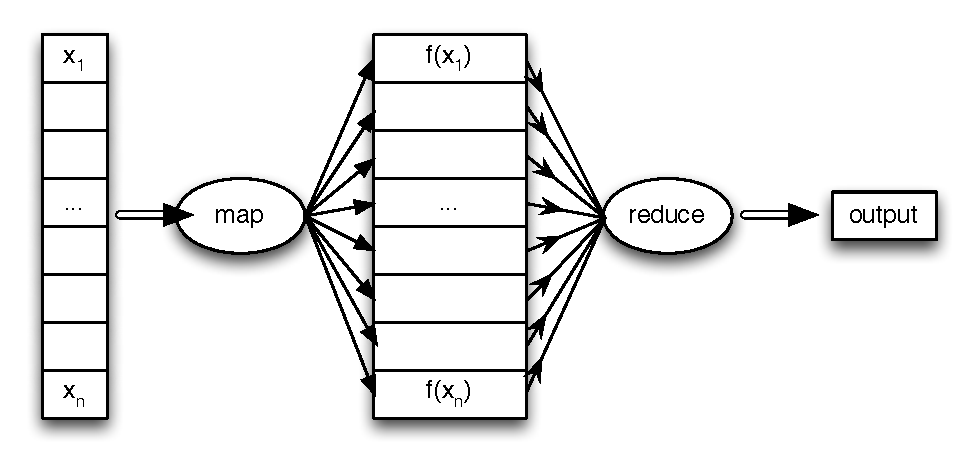
\includegraphics[width=2.5in]{images/mapreduce}
  % \hspace{30px}
  \hfill
	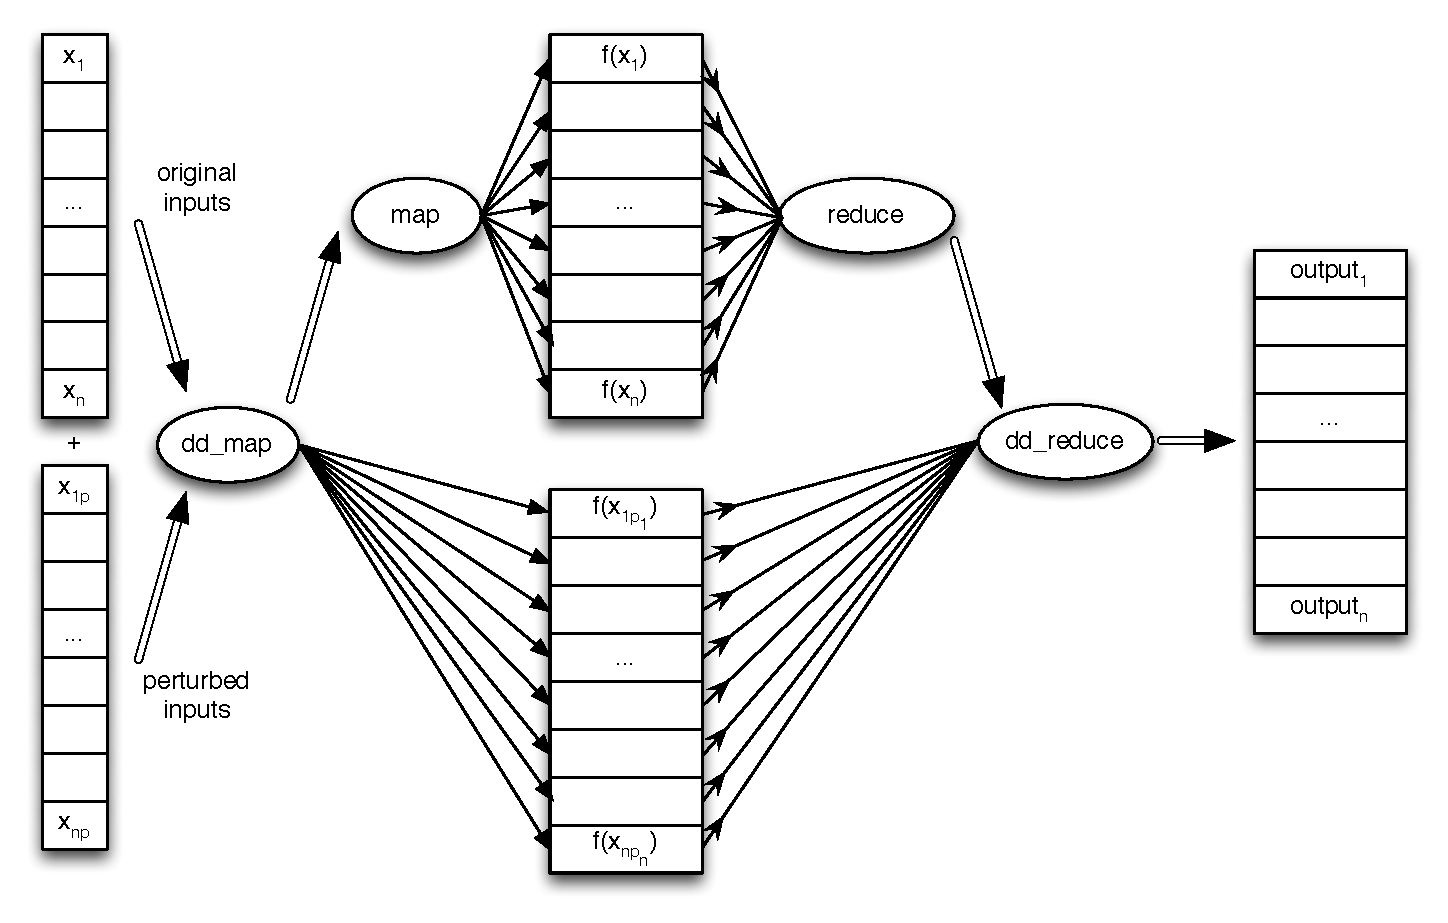
\includegraphics[width=3.25in]{images/mapreduce_dd}
	\caption{
		On the left, a typical MapReduce job.  On the right, a data debug-augmented MapReduce job.  Each additional output is a version of the computation with the unusually impactful values automatically excluded.\label{fig:mapreduce_pipeline}
	}
\end{figure*}

\paragraph{MapReduce-Based Frameworks.}
While MapReduce and Hadoop jobs are low-level programming idioms,
frameworks like FlumeJava (and by extension, its Hadoop-based clone, Crunch)
allow multi-stage MapReduce programs to be represented by higher-level
programming constructs~\cite{pldi:flumejava}.  These constructs allow
the runtime to determine a program dependency graph.  This
higher-level representation gives the runtime global information that
facilitates automatic performance-enhancing program transformations,
such as reordering of functions in the program call graph to increase
parallelism.

We observe that data-parallel programs constructed in this fashion
share many of the same properties that make data debugging a useful
technique in spreadsheets.  The input to the mapper stage of a
MapReduce problem is a large, homogeneous vector amenable to the same
kind of input perturbation that \checkcell{} employs.  A key property
of the computation kernel in a MapReduce job is that code be
shared-nothing and re-entrant. Therefore, data debugging (which often
needs to recompute certain portions of the call graph) can be inserted
into a portion of a MapReduce job without affecting the semantics of
the original program.

\paragraph{Data Debugging for Robustness.}
As with \checkcell{}, data debugging functions can transparently
augment a FlumeJava program.  The tradeoff is a small performance
penalty for the additional robustness data debugging provides. Data
debugging techniques can be piggybacked on a high-level representation
so that impact analysis can take advantage of underutilized
parallelism to minimize the performance impact of our technique.

To be feasible, large-scale data debugging requires at least two kinds
of program transformations.  First, a data debugging-enhanced library
like FlumeJava would augment the map stage with perturbed input values
to be computed in parallel, and the reducer function would be
augmented with the impact computation.  Our implementation of
\checkcell{} relies on Microsoft Excel's ability to recognize when
partial recomputation of the dependency graph is possible for
efficiency purposes. A data debugging-enhanced FlumeJava runtime would
need to recognize when an impact calculation may be performed for
only a subset of the program dependency graph, and when the dependency
analysis itself contains overlapping subproblems whose solutions
should be shared to improve performance.

Once impact scores are known for a set of MapReduce program inputs,
the data debugging runtime can be instructed to re-run the computation
with the unusually impactful inputs either removed or replaced with
user-specfied values.  The degree of unusualness, in terms of standard
deviations from the norm, may be used to control the degree of
input trimming performed on the MapReduce input vector.  Again,
a high-level representation of the program graph allows this
recomputation to be performed for the minimum cost possible.
